\documentclass[conference]{IEEEtran}

\usepackage{cite}
\usepackage{amsmath,amssymb}
\usepackage{graphicx}
\graphicspath{{./}{figures/}}
\usepackage{booktabs}
\usepackage{url}
\usepackage{tikz}
\usetikzlibrary{arrows.meta}

\begin{document}

\title{Qwen3-ASR-1.7B for Speech-to-Text:\\Architecture Analysis and Experimental Evaluation}

\author{\IEEEauthorblockN{Nagham Taweel}
\IEEEauthorblockA{NLP \& AI Internship, Cellula Technologies\\
naghamatawel@gmail.com}}

\maketitle

\begin{abstract}
Qwen3-ASR-1.7B is an open-source automatic speech recognition (ASR) model from the Qwen Team that combines a 300M-parameter audio encoder with the Qwen3-1.7B language model and supports 52 languages and dialects. This report analyzes its architecture and training, and evaluates it experimentally by running the official \texttt{qwen-asr} package on an Apple M4 Pro laptop. We built a 72-clip test set (19.7 minutes, 2,980 reference words) from LibriSpeech, EdAcc, and FLEURS that covers different speakers, 12 English accents, Egyptian Arabic, added noise from 20 to 0\,dB, and recordings up to 5 minutes long. We measured word and character error rates, processing time, and memory, and compared the model with Qwen3-ASR-0.6B and Whisper large-v3-turbo. Qwen3-ASR-1.7B achieved 1.2\% WER on clean speech, 10.6\% on accented conversation, 10.8\% WER (2.7\% CER) on Arabic, and 7.3\% at 0\,dB, the best result under heavy noise. On the laptop's GPU it ran about ten times faster than real time with 9\,GB of memory. All results come from actual runs of the model.
\end{abstract}

\begin{IEEEkeywords}
automatic speech recognition, Qwen3-ASR, Whisper, word error rate, multilingual speech, robustness
\end{IEEEkeywords}

\section{Introduction}
Speech-to-text (STT) systems convert spoken audio into written text and are used in voice assistants, meeting transcription, and accessibility tools. Recent systems such as Whisper~\cite{whisper} showed that a single model trained on very large, weakly labeled data can transcribe many languages. Qwen3-ASR, described by the Qwen Team in a January 2026 technical report and released under the Apache 2.0 license, follows a different design: it attaches an audio encoder to a large language model (LLM)~\cite{qwen3asr,qwen3asrgit}. It comes in two sizes, 1.7B and 0.6B, and supports 30 languages and 22 Chinese dialects, language identification, and audio up to 20 minutes~\cite{qwen3asr}.

This report has two goals: to explain how Qwen3-ASR-1.7B works, and to test it in practice on speech that differs in speaker, accent, language, noise, and duration. All numbers in Sections~V and VI come from our own runs.

\section{Architecture Analysis}
\textbf{Pipeline.} Fig.~\ref{fig:pipe} shows the model. Audio sampled at 16\,kHz is converted to 128-dimensional log-Mel filter-bank (Fbank) features. The AuT encoder, an attention-based encoder with 300M parameters and a hidden size of 1024, downsamples these features by 8 to produce audio tokens at 12.5\,Hz~\cite{qwen3asr}. One second of speech therefore becomes 12.5 tokens, so a 5-minute recording becomes 3,750 tokens. A projector maps the audio tokens into the embedding space of Qwen3-1.7B~\cite{qwen3}, which generates the language tag and the transcript token by token:
\begin{equation}
P(y\mid\mathbf{x})=\prod_{t=1}^{T}P_\theta\!\left(y_t\mid y_{<t},\,\mathrm{Proj}(\mathrm{AuT}(\mathbf{F}(\mathbf{x})))\right),
\end{equation}
where $\mathbf{x}$ is the waveform, $\mathbf{F}$ the Fbank features, and $y$ the output text. Because the decoder is a full LLM, it brings strong language knowledge, which helps with names, rare words, and punctuation. The encoder uses a dynamic attention window from 1 to 8\,s, so the same model supports streaming with short chunks and offline transcription of long files~\cite{qwen3asr}.

\begin{figure}[t]
\centering
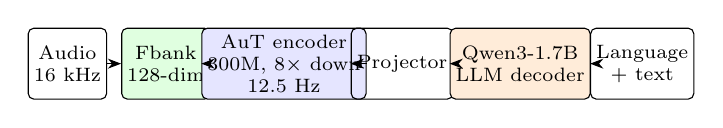
\begin{tikzpicture}[font=\scriptsize, >=Stealth,
  b/.style={draw, rounded corners=2pt, align=center, minimum height=0.9cm, inner sep=2pt}]
\node[b] (a) at (0,0) {Audio\\16 kHz};
\node[b, fill=green!12] (f) at (1.25,0) {Fbank\\128-dim};
\node[b, fill=blue!10] (e) at (2.75,0) {AuT encoder\\300M, $8\times$ down\\12.5 Hz};
\node[b] (p) at (4.25,0) {Projector};
\node[b, fill=orange!15] (l) at (5.75,0) {Qwen3-1.7B\\LLM decoder};
\node[b] (o) at (7.3,0) {Language\\+ text};
\draw[->] (a) -- (f);
\draw[->] (f) -- (e);
\draw[->] (e) -- (p);
\draw[->] (p) -- (l);
\draw[->] (l) -- (o);
\end{tikzpicture}
\caption{Qwen3-ASR-1.7B pipeline, based on~\cite{qwen3asr}.}
\label{fig:pipe}
\end{figure}

\textbf{Training.} Training has four stages~\cite{qwen3asr}. First, the AuT encoder is pre-trained on about 40 million hours of pseudo-labeled speech, mostly Chinese and English. Second, the full model is pre-trained on 3 trillion tokens, following Qwen3-Omni. Third, supervised fine-tuning on a smaller multilingual set teaches the transcription style, and adds non-speech, streaming, and context-biasing data. Finally, reinforcement learning with group sequence policy optimization (GSPO) on about 50k utterances further reduces errors.

\textbf{Reported results.} The technical report gives Qwen3-ASR-1.7B a WER of 1.63/3.38\% on LibriSpeech test-clean/other, compared with 1.51/3.97\% for Whisper-large-v3. On accented English dialogs the WERs are 16.07\% vs.\ 21.30\%, and on an extreme-noise set 16.17\% vs.\ 63.17\%~\cite{qwen3asr}. With vLLM on a data-center GPU, the 1.7B model reaches a real-time factor of 0.015 at a concurrency of 1~\cite{qwen3asr}.

\section{Experimental Setup}
\textbf{Test set.} Table~\ref{tab:data} lists the 72 clips, each with a human reference transcript. We took one utterance per speaker from LibriSpeech test-clean and test-other~\cite{librispeech}, one utterance per accent from the EdAcc conversational corpus~\cite{edacc}, and read sentences in Egyptian Arabic and US English from FLEURS~\cite{fleurs}. To vary recording conditions, we added white Gaussian noise to five clean clips at signal-to-noise ratios (SNR) of 20, 10, 5, and 0\,dB. To vary duration, we joined consecutive LibriSpeech utterances into recordings of 47, 72, 124, and 305\,s. All clips are 16\,kHz mono.

\textbf{Metrics.} The word error rate is
\begin{equation}
\mathrm{WER}=\frac{S+D+I}{N},
\end{equation}
where $S$, $D$, and $I$ are substituted, deleted, and inserted words and $N$ is the number of reference words. The character error rate (CER) applies the same formula to characters and is fairer for Arabic, where small spelling differences count as whole-word errors. Before scoring, both texts are normalized with the Whisper English normalizer, or with its basic normalizer for Arabic, which also removes diacritics. Errors are summed over all clips in a group. The real-time factor $\mathrm{RTF}=t_{\mathrm{proc}}/t_{\mathrm{audio}}$ measures speed; values below 1 are faster than real time.

\textbf{Systems.} We compared Qwen3-ASR-1.7B and Qwen3-ASR-0.6B with Whisper large-v3-turbo~\cite{whisper}, all with automatic language detection and greedy decoding.

\begin{table}[t]
\centering
\caption{Test set built for the experiments}
\label{tab:data}
\setlength{\tabcolsep}{3pt}
\begin{tabular}{llrrr}
\toprule
Group & Condition & Clips & Audio (s) & Words \\
\midrule
LibriSpeech clean & read, 10 speakers & 10 & 92 & 243 \\
LibriSpeech other & harder audio, 10 speakers & 10 & 109 & 288 \\
FLEURS en-US & read, US English & 8 & 70 & 156 \\
EdAcc & conversation, 12 accents & 12 & 90 & 170 \\
FLEURS ar-EG & read, Egyptian Arabic & 8 & 91 & 158 \\
Noise & SNR 20/10/5/0 dB & 20 & 180 & 496 \\
Duration & 47--305 s recordings & 4 & 548 & 1{,}469 \\
\midrule
Total & & 72 & 1{,}181 & 2{,}980 \\
\bottomrule
\end{tabular}
\end{table}

\section{Implementation Details}
Experiments ran on a MacBook with an Apple M4 Pro chip and 26\,GB of unified memory, using Python 3.12, \texttt{qwen-asr} 0.0.6, PyTorch 2.15, and Transformers 4.57.6 in an isolated environment, as the official guide recommends~\cite{qwen3asrgit}. The model was loaded with \texttt{Qwen3ASRModel.from\_pretrained}, which downloads 4.7\,GB of BF16 weights, and called through \texttt{transcribe(audio, language=None)}, which returns the detected language and the text. The official examples target NVIDIA GPUs (\texttt{device\_map="cuda:0"})~\cite{qwen3asrgit}. Setting \texttt{device\_map="mps"} ran the model on the Apple GPU in BF16 without code changes, and \texttt{"cpu"} ran it in FP32. We used a batch size of 1 and up to 2,048 new tokens. Whisper ran through faster-whisper~\cite{fasterwhisper} with INT8 weights on the CPU, since it does not support the Apple GPU. Timing used a warm-up call and GPU synchronization, and memory was read from the process and the MPS driver.

Two practical problems appeared. Python from python.org could not verify HTTPS certificates when downloading audio, which we fixed by pointing \texttt{SSL\_CERT\_FILE} to the \texttt{certifi} bundle. The installed faster-whisper version was also incompatible with its audio decoding library, so we passed decoded arrays instead of file paths.

\section{Results and Discussion}
\textbf{Accuracy.} Table~\ref{tab:wer} shows WER and CER per group. On clean read English, all systems are below 2\% WER, and Whisper is slightly better on LibriSpeech clean (0.82\% vs.\ 1.23\%). Qwen3-ASR-1.7B is best on FLEURS English (2.56\%), accented conversation (10.59\%), and Arabic (10.76\% WER, 2.65\% CER). The Arabic gap between WER and CER shows that most Arabic errors are small spelling variants, such as a missing long vowel or a different gender ending, rather than wrong words. The 0.6B model is close to the 1.7B model in English but clearly worse in Arabic (16.46\%). Every one of the 226 transcriptions in our four runs identified the language correctly.

\begin{table}[t]
\centering
\caption{Measured WER / CER (\%) per group}
\label{tab:wer}
\setlength{\tabcolsep}{3pt}
\begin{tabular}{lccc}
\toprule
Group & Qwen3-ASR-1.7B & Qwen3-ASR-0.6B & Whisper-turbo \\
\midrule
LibriSpeech clean & 1.23 / 0.45 & 1.65 / 0.53 & \textbf{0.82} / 0.30 \\
LibriSpeech other & \textbf{0.69} / 0.13 & \textbf{0.69} / 0.33 & 1.04 / 0.47 \\
FLEURS en-US & \textbf{2.56} / 0.77 & 3.85 / 1.54 & 4.49 / 1.43 \\
EdAcc accents & 10.59 / 7.41 & \textbf{10.00} / 8.06 & 12.94 / 9.36 \\
FLEURS ar-EG & \textbf{10.76} / 2.65 & 16.46 / 3.75 & 12.03 / 3.53 \\
Noise (all SNR) & \textbf{3.63} / 1.87 & 6.05 / 3.60 & 5.04 / 2.72 \\
Duration & 3.54 / 1.68 & 7.42 / 3.68 & \textbf{1.77} / 0.67 \\
\bottomrule
\end{tabular}
\end{table}

\begin{figure*}[t]
\centering
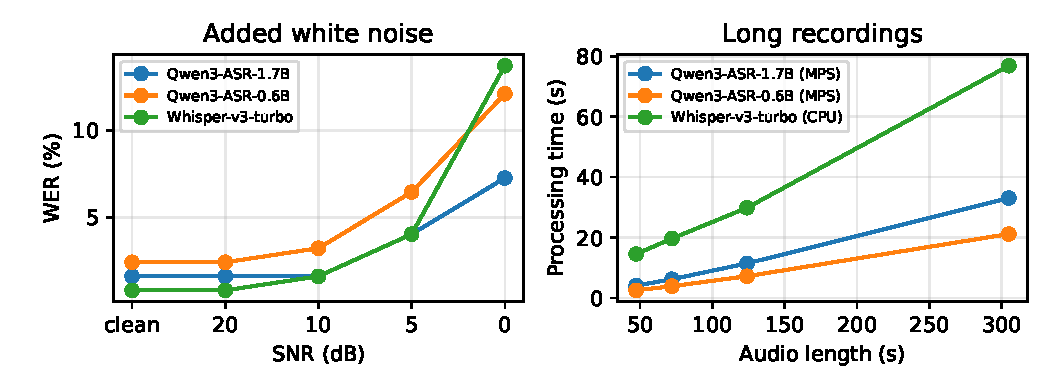
\includegraphics[width=0.8\textwidth]{results.pdf}
\caption{Measured WER under added white noise (left) and processing time for long recordings (right). Qwen3-ASR runs on the Apple GPU (MPS) and Whisper on the CPU.}
\label{fig:results}
\end{figure*}

\textbf{Accents.} Per-accent results vary widely. Scottish, US, Eastern European, Latin American, and Bulgarian speakers were transcribed with no errors by Qwen3-ASR-1.7B, while Whisper made errors on the Scottish and US clips. The hardest clips were short utterances of participant codes. For a Romanian speaker, the reference ``I am participant C nine P one'' was recognized as a name followed by ``9B1'' (71\% WER), and for a Spanish speaker the model wrote the filler word ``vale'', which the reference omits, and confused the letter C with P. These are short, context-free sequences, where the language model cannot help (Table~\ref{tab:examples}). In the Nigerian example, the only error is that the letters ``F C'' were joined into ``FC''.

\textbf{Noise.} Fig.~\ref{fig:results} (left) shows that Qwen3-ASR-1.7B was unaffected down to 10\,dB SNR (1.61\% WER) and reached 7.26\% at 0\,dB, where the noise is as loud as the speech. Whisper started better (0.81\%) but rose to 13.71\% at 0\,dB, and the 0.6B model to 12.10\%. This matches the robustness reported in~\cite{qwen3asr}.

\textbf{Duration and speed.} Processing time grew roughly linearly with audio length (Fig.~\ref{fig:results}, right). The 305\,s recording took 33.1\,s with Qwen3-ASR-1.7B on the GPU, with 5.54\% WER. Its errors were scattered single words in harder passages, not skipped segments. Table~\ref{tab:speed} summarizes speed and memory. On the Apple GPU, the 1.7B model processed the whole test set at an RTF of 0.10, about ten times faster than real time, using 9.0\,GB of GPU memory. The 0.6B model was 1.6 times faster with 6.3\,GB. On the CPU, the 1.7B model in FP32 still reached an RTF of 0.24 on the ten LibriSpeech-clean clips, faster than Whisper-turbo in INT8 on the same clips (RTF 1.00). Whisper processes audio in fixed 30\,s windows, which is costly for short clips. Our laptop RTF of 0.10 is about seven times slower than the 0.015 reported with vLLM on a data-center GPU~\cite{qwen3asr}, as expected for unoptimized single-stream inference.

\begin{table}[t]
\centering
\caption{Measured speed and memory}
\label{tab:speed}
\setlength{\tabcolsep}{3pt}
\begin{tabular}{llccc}
\toprule
System & Device & Clips & RTF & Peak memory \\
\midrule
Qwen3-ASR-1.7B & MPS, BF16 & 72 & 0.101 & 9.0 GB (GPU) \\
Qwen3-ASR-0.6B & MPS, BF16 & 72 & \textbf{0.063} & 6.3 GB (GPU) \\
Whisper-turbo & CPU, INT8 & 72 & 0.658 & 2.9 GB (RAM) \\
Qwen3-ASR-1.7B & CPU, FP32 & 10 & 0.241 & 9.4 GB (RAM) \\
Whisper-turbo & CPU, INT8 & 10 & 1.001 & 2.9 GB (RAM) \\
\bottomrule
\end{tabular}
\end{table}

\begin{table}[t]
\centering
\caption{Input/output examples from Qwen3-ASR-1.7B}
\label{tab:examples}
\setlength{\tabcolsep}{3pt}
\begin{tabular}{p{1.55cm}p{5.35cm}r}
\toprule
Audio & Reference (R) and model output (O) & WER \\
\midrule
LibriSpeech, 0\,dB noise & R: concord returned to its place amidst the tents \newline O: Concord returned to its place amidst the tents. & 0.0 \\
EdAcc, Nigerian English & R: okay um my participant number is f c nineteen p one how about you \newline O: Okay. Um, my participant number is FC nineteen P one. How about you? & 15.4 \\
EdAcc, Romanian accent & R: I am participant C nine P one \newline O: Okay. Hi, I'm Brita Spindzic, 9B1. & 71.4 \\
\bottomrule
\end{tabular}
\end{table}

\textbf{Limitations and improvements.} The test set is small (2,980 words), so differences below about one point are not significant. This explains why LibriSpeech-other scored lower than LibriSpeech-clean here, unlike in the official results. The noise is synthetic white noise rather than real background sound, the speed comparison mixes devices because Whisper cannot use the Apple GPU, and Arabic was tested only on read Egyptian speech. Future work should use larger sets with real noise and spontaneous Arabic dialects, add timestamps with the Qwen3-ForcedAligner, and test vLLM serving on a CUDA GPU.

\section{Conclusion}
Qwen3-ASR-1.7B combines an AuT audio encoder with a Qwen3 LLM decoder. In our experiments on a laptop, it transcribed clean English almost perfectly, handled accents, Arabic, and heavy noise better than Whisper large-v3-turbo, identified every language correctly, and ran ten times faster than real time on the Apple GPU. Its main weaknesses are short, context-free utterances such as codes and names, and a memory cost of about 9\,GB. The 0.6B version is a good alternative for English when speed matters.

\bibliographystyle{IEEEtran}
\bibliography{references}

\end{document}
